%\documentclass[11pt,a4paper,bibtotoc]{scrartcl}
\documentclass[journal]{IEEEtran}
%\documentclass[11pt,a4paper,twoside]{article}
%\usepackage[T1]{fontenc}
%\usepackage[latin1]{inputenc}
\usepackage[english]{babel}
\usepackage{amsmath}%\usepackage{amsthm}
\usepackage{amssymb}
\usepackage{graphics}
%\usepackage{showkeys}
\usepackage{times}
\usepackage{alltt}
\usepackage{latexsym}
%\usepackage{pstricks}
\usepackage{graphicx}
\usepackage{cite}
\def\ti{\mbox{\scriptsize{\rm i}}}
%\newcommand{\eipp}[1]{{\rm e}^{ \pi{\ti} #1}}
%\newcommand{\eimp}[1]{{\rm e}^{- \pi{\ti} #1}}
\newcommand{\eip}[1]{{\rm e}^{ 2\pi{\ti} #1}}
\newcommand{\eim}[1]{{\rm e}^{-2\pi{\ti} #1}}
\newcommand{\zb}[1]{\mbox{\boldmath{${#1}$}}}
\newcommand{\zbs}[1]{\mbox{\boldmath\scriptsize{${#1}$}}}
\newcommand{\zbss}[1]{\mbox{\boldmath\tiny{${#1}$}}}
\newcommand{\dist}{{\rm dist}}
\newcommand{\cond}{{\rm cond}}
\newcommand{\diag}{{\rm diag}}
\renewcommand{\mod}{\;{\rm mod}\;}
\renewcommand{\d}{{\rm d}}
\newcommand{\supp}{{\rm supp}}
\newcommand{\card}{{\rm card}}
\newcommand{\adj}{{\vdash \hspace*{-1.72mm} \dashv}}

\renewcommand{\Box}{\hspace*{0ex} \hfill \rule{1.5ex}{1.5ex} \\ \goodbreak}
\newcommand{\Boxgl}{\par\vspace{-5ex} \hspace*{0ex} \hfill
  \rule{1.5ex}{1.5ex} \\ \goodbreak\goodbreak}
\newcommand{\bend}{\hspace*{0ex} \hfill \hbox{\vrule height
    1.5ex\vbox{\hrule width 1.4ex \vskip 1.4ex\hrule  width 1.4ex}\vrule
    height 1.5ex} \goodbreak}
\newtheorem{theorem}{Theorem}[section]
\newtheorem{lemma}[theorem]{Lemma}
\newtheorem{remark}[theorem]{Remark}
\newtheorem{definition}[theorem]{Definition}
\newtheorem{example}[theorem]{Example}
\newtheorem{corollary}[theorem]{Corollary}
\newtheorem{algorithm}[theorem]{Algorithm}

\newenvironment{Theorem}{\goodbreak \begin{theorem}\sl}{\end{theorem}}
\newenvironment{Lemma}{\goodbreak \begin{lemma}\sl}{\end{lemma}}
\newenvironment{Remark}{\goodbreak \begin{remark}\rm}{\hfill \bend\end{remark}}
\newenvironment{Example}{\goodbreak \begin{example}\rm}{\hfill \bend \end{example}}
\newenvironment{Definition}{\goodbreak \begin{definition}\rm}{\end{definition}}
\newenvironment{Corollary}{\goodbreak \begin{corollary}\rm}{\end{corollary}}
\newenvironment{Algorithm}{\begin{algorithm}\sl}{\hfill
  \end{algorithm}}

\renewcommand{\labelenumi}{\roman{enumi})} %aendert die Label
%\renewcommand{\theequation}{\arabic{section}.\arabic{equation}}

\numberwithin{equation}{section}
\numberwithin{table}{section}
\numberwithin{figure}{section}

\setcounter{totalnumber}{10}
\setcounter{topnumber}{10}

\title{Image reconstruction for MRI in the Presence of
  Filed Inhomogeneties}

\author{
Holger Eggers\thanks{\tt Philips},
Tobias Knopp\thanks{University of L\"ubeck,
Institute of Mathematics,
D--23560 L\"ubeck,
Germany, {\tt tobias.knopp@informatik.uni-luebeck.de}}, 
Daniel Potts\thanks{University of L\"ubeck,
Institute of Mathematics,
D--23560 L\"ubeck,
Germany, {\tt potts@math.uni-luebeck.de}}
}

\begin{document}

%\date{}

\maketitle

%\markboth{Journal of \LaTeX\ Class Files,~Vol.~1,
%No.~11,~November~2002}{Shell \MakeLowercase{\textit{et al.}}: Bare
%Demo of IEEEtran.cls for Journals} 

\begin{abstract}

\end{abstract}

2000 {\it Mathematics Subject Classification} 65T50, 68U10

%{\it Key words and phrases:} 
\begin{keywords}
2d/3d image reconstruction, iterative methods, magnetic resonance imaging, Fourier transform, FFT, NFFT, gridding, rose scan, spiral scan.
\end{keywords}


%------------------------------------------------------------------------------
\section{Introduction}
% Hier sollte motivert werden, warum die Inhomogenti�ten wieder interessant werden:
% k�rzere R�hren? usw.
\section{Theory}\label{Sec:Th}

In MRI, ignoring relaxation effects, the relation between the MR signal
$s_{\text{MR}}$ during the readout and the object $\tilde p$ can be modelled by
\begin{equation}\label{signal_eq}
s_{\text{MR}}\left(t\right) =
\int_{\mathbb{R}^3} \tilde p \left(\zb r\right) c\left(\zb r\right)
{\rm e}^{{\rm\scriptsize i}\omega(\zbs r)(t+T_E)}
{\rm e}^{2\pi {\rm\scriptsize i}\zbs r \zbs k\left(t\right)} \d \zb r\, ,
\end{equation}
where $T_E$ is the echo time,  
$c\left(\zb r\right)$ is the known sensitivity of the receiver coil,
$\omega(\zb r)$ is the field inhomogeneity present at $\zb r$, 
and
$\zb k(t)$ is the k-space trajectory.
%see \cite{SuNoFe03} for a low rank approximation of these effects.
We follow \cite{SuNoFe03}  and let for simplicity
$$
p(\zb r)= \tilde p(\zb r) c(\zb r) 
{\rm e}^{{\rm\scriptsize i}\omega(\zbs r)T_E}\, .
$$
Accurate estimation of $p(\zb r)$ yield $\tilde p(\zb r)$ assuming the
sensitivity and field maps are known.
For convenience let the available samples in k-space be contained in the shifted unit square, i.e.
$\zb k \in [-\frac{1}{2},\frac{1}{2})^2$, and the field of view be restricted to 
$\Omega_{\zbs N} \subset [-\frac{N_1}{2},\frac{N_1}{2})\times[-\frac{N_2}{2},\frac{N_2}{2})$,
where $\zb N=(N_1,N_2)^{\top} \in 2\mathbb{N}^2$.
Then, the discretisation of integral \eqref{signal_eq} on equispaced points leads to
\begin{equation}\label{inverse2}
s(\zb k(t)) \approx \tilde{s}(\zb k(t)) := \sum_{\zbs r \in I^2_{\zbss
    N}} p(\zb r) 
{\rm e}^{{\rm\scriptsize i}\omega(\zbs r)t}
{\rm e}^{2\pi {\rm\scriptsize i}\zbs r \zbs k(t)}
\, ,
\end{equation}
where $I^2_{\zbs N} :=
\{-\frac{N_1}{2},\dots,\frac{N_1}{2}-1\}\times\{-\frac{N_2}{2},\dots,
\frac{N_2}{2}-1\}$.

We denote the vector of the given values by $\zb {s}:=(\tilde s({\zb k_j}))_{j=0,\ldots,M-1}\in \mathbb{C}^{M}$,
the reshaped vector of the unknown object by $\zb {p}:=(p({\zb r}))_{\zbs r\in I_{\zbss N}^2} \in
\mathbb{C}^{N_1\times N_2}$ and the matrix 
\begin{equation}\label{MatrixB}
\zb H:=\left({\rm e}^{{\rm\scriptsize i}\omega(\zbs r)t_j} \eip{\zbs r\zbs k(t_j)}\right)_{j=0,\hdots,M-1;\;\zbs r\in
  I_{\zbss N}^2}\, ,
\end{equation}
Thus, the unknown object $p$ is given {\em implicit} by \eqref{inverse2}.
The authors of \cite{DeWaLe02} call this inverse model.
We propose to solve this system of linear equations by weighted least
squares, where the 
weights $w_j> 0$ compensate for clusters in the sampling set, i.e.,
\begin{equation} \label{eq:min}
  \|\zb s - \zb H \zb  p\|_{\zbs W}
  = \left(\sum_{j=0}^{M-1} w_j |s(\zb k_j)-\tilde s(\zb k_j)|^2\right)^{1/2}
  \stackrel{\zbs {\hat f}}{\rightarrow} \min,
\end{equation}
where $\zb W:=\diag(w_j)_{j=0,\ldots,M-1}$.
This problem is equivalent to the weighted normal equation of first kind
\begin{equation}
  \label{eq:no1}
  \zb H^{\adj} \zb W \zb H \zb {\hat f} = \zb H^{\adj} \zb W \zb y.
\end{equation}
The iterative solution of problem \eqref{eq:no1} can be solved 
by a suitable variant of conjugated gradients (CGNR). 

We state problem \eqref{inverse2} as the weighted approximation problem
\begin{equation}\label{minMR}
  \|\zb s - \zb {\tilde s}\|_{\zbs W}
  \stackrel{\zbs {p}}{\rightarrow} \min,
\end{equation}
where $\zb {\tilde s}=\zb H\zb p$, see \eqref{inverse2}, and the density compensation weights are collected in the diagonal matrix
$\zb W=\diag(w_j)_{j=0,\ldots,M-1}$. 
We would like to emphasise that the CGNR method minimises \eqref{minMR} in each iteration over a certain Krylov space.
Thus, iterate for only one step, we obtain the 'optimised' gridding
solution.
An algorithm for the fast multiplication with the matrix $\zb H$ and
$\zb H^{\top}$  is the key for CGNR and so for a fast solution of \eqref{inverse2}.

\section{NFFT}\label{Sec:NFFT}

If the data are sampled on a Cartesian grid in k-space the
reconstruction can be done with the FFT. For non-Cartesian
trajectories in k-space the reconstruction can be done via
\eqref{inverse2}, where the FFT has to be replaced by the NFFT.

In the following we briefly describe the NFFT, which has, for a fixed accuracy,
the same arithmetical complexity as the FFT. One can use the
software package, which is available from the NFFT homepage \cite{kupo02C}.

The NFFT can be introduced as follows. 
Let $\varphi\in L^2(\mathbb{R})\cap L^1(\mathbb{R}) $ given, such that
the one periodisation
\begin{equation} \label{phiper}
\tilde\varphi(x) :=  \sum_{r=-\infty}^{\infty} \varphi(x+r)
\end{equation} 
has a uniformly convergent Fourier series.
Hence we write the function $\tilde\varphi$ as Fourier series 
\begin{equation} \label{FRphi}
\tilde\varphi (x) =  \sum_{ k=-\infty }^{\infty}  c_{k}(\tilde\varphi)  
\eip{ k x} 
\end{equation} 
with the Fourier coefficients 
\begin{equation} \label{FKphi}
c_{ k} (\tilde \varphi ) :=  
\int\limits_{-1/2}^{1/2} \tilde\varphi ( x)
  \eim{ kx} \, {\rm d} {x} \quad ( k \in \mathbb{Z}) 
\end{equation}
and we obtain 
\begin{equation}\label{FK=ck}
\hat\varphi(k) := \int\limits_{-\infty}^{\infty} \varphi ( x)
  \eim{ k x} \, \d { x} = c_{ k} (\tilde \varphi )\, .
\end{equation}
The Fourier coefficients
\begin{equation} \label{FKphi}
c_{ k} (\tilde \varphi ) =  
\int\limits_{-\infty}^{\infty} \tilde\varphi (x-y)
  \eim{ k(x-y)} \, {\rm d} {y} \quad ( k \in \mathbb{Z}, x\in[-1/2,1/2)) 
\end{equation}
can be approximated for $k=-N/2,\ldots, N/2-1$ by
\begin{equation} \label{approx}
c_{ k} (\tilde \varphi ) \approx
\frac{1}{\alpha N} \sum_{l=-\alpha N/2}^{\alpha N/2-1}
\tilde\varphi (x-\frac{l}{\alpha N})  \eim{ k(x-\frac{l}{\alpha N})} \,
\end{equation}
with an oversampling factor $\alpha >1$.
But \eqref{approx} can be written as
\[
c_{ k} (\tilde \varphi ) \approx
\frac{1}{\alpha N}\eim{kx}
\sum_{l=-\alpha N/2}^{\alpha N/2-1}
\tilde\varphi (x-\frac{l}{\alpha N})  \eim{\frac{kl}{\alpha N}} \,,\quad
\]
and further for $k=-N/2,\ldots,N/2$
\begin{equation} \label{approx}
\eip{kx}
\approx
\frac{1}{nc_{ k} (\tilde \varphi )}
\sum_{l=-n/2}^{n/2-1}
\tilde\psi (x-\frac{l}{\alpha N})  \eim{\frac{kl}{\alpha N}}
\end{equation}
where $\tilde\psi$ is the one periodisation 
$
\displaystyle\tilde\psi(x) := \sum_{r=-\infty}^{\infty} \psi(x +r)\,
\in L^2(\mathbb{T})
$
and $\psi$ the truncation of $\varphi$, i.e.
\begin{equation}\label{Defpsi}
\psi(x) := \left\{
\begin{array}{ll}
\varphi(x) & \textrm{if }  x \in [- m/n,m/n], \\
0 & \textrm{else},
\end{array} \right.
\end{equation}
with a truncation parameter $m$ $(m\ll N,m\in \mathbb{N})$. 
Note that the approximation of the exponentials in \eqref{approx} is
used in order to develop the NFFT. The methods differ only by choosing
different window functions $\varphi$. 
For a finite number of  
given Fourier coefficients $\hat f_{k} \in \mathbb{C}$
we want to
evaluate the trigonometric polynomial  
\begin{equation}
 \label{trigPoly}
  f\left( x\right) := \sum_{k=-N/2}^{N/2-1} \hat{f}_{k} \eip{ k x}
\end{equation}
at given non equispaced knots $ x_j \in
[-\frac{1}{2},\frac{1}{2})^d,\;j=0,\hdots,M-1$. 
Thus, our concern is the fast evaluation of
\begin{equation*}
 f_j = \sum_{k=-N/2}^{N/2-1} \hat{f}_{k} \eip{k x_j}\,, \qquad
 j=0,\hdots,M-1. 
\end{equation*}
Using now the approximation of the exponentials given in \eqref{approx}
we obtain
\begin{equation}
 \label{NFFTapr}
f_j \approx\sum_{l=-\alpha N/2}^{\alpha N/2-1}\left(
\sum_{ k=-N/2}^{N/2-1} \frac{\hat{f}_{k}}{\alpha N c_{k} (\tilde \varphi )}
\eim{\frac{kl}{\alpha N}}
\right)\tilde\psi (x_j-\frac{l}{\alpha N})  \, .
\end{equation}
In matrix vector notation \eqref{trigPoly} reads as
\begin{equation}
 \label{ndft}
 \zb f=\zb A \zb {\hat f}
\end{equation}
where 
\begin{equation*}
\zb A:=\left(\eim{k x_j}\right)_{j=0,\hdots,M-1;\;k=-N/2,\ldots,N/2-1}\, ,
\end{equation*}
\begin{equation*}
\zb f:=\left(f_j\right)_{j=0,\hdots,M-1},\quad 
\zb {\hat f}:=\left(\hat{f}_{\zbs r}\right)_{\zbs r\in I_{\zbss N}^d}.
\end{equation*}
and the approximation \eqref{NFFTapr} to a fast
evaluation of \eqref{trigPoly} can
be written as 
$\zb A \approx \zb B \zb F \zb D$ with a diagonal matrix $\zb
D=\diag(\hat \varphi(\zb r))$,
an oversampled Fourier matrix $\zb F$, and
a sparse matrix $\zb B$
with nonzero entries $b_{j,l}=\psi (\zb x_j - l/ (\alpha N))$, where
$\psi$ approximates the window  function $\varphi$ and $\alpha$
denotes the oversampling factor. The generalisation to higher
dimensions is straightforward. A unified approach to the
efficient computations of \eqref{trigPoly} was suggested in \cite{st97,
  postta01}. It was already pointed out in \cite{postta01,SaBeCo01},
that the gridding 
method is simply a fast algorithm for the multiplication of the matrix
$\zb A^{\adj}$ with a vector (see also \cite{KnKuPo}).
Our algorithms are based on the approach in \cite{postta01} where one can change 
the window function $\varphi$ in a very simple way. Note, that
\begin{enumerate}
\item For a fixed oversampling factor $\alpha >1$ the approximation error introduced by the NFFT
decays exponentially with the window-width $m$.
\item The arithmetical complexity of the NFFT is ${\cal O} ((\alpha N)^d\log N+m^d M)$. 
\end{enumerate}
The manual \cite{kupo04b} and the appendix in \cite{post02} present details
for a suitable choice of the window function, the window-width, and the
oversampling factor with respect to accuracy, speed and memory usage.


Since the support of $\tilde\psi$ is ${\rm supp} \tilde\psi\subset
[-m/(\alpha N), m/(\alpha N)]$ we can avoid the periodisation of $\psi$ 
if $x\in[-\frac{1}{2}+\frac{m}{\alpha N},-\frac{1}{2}+\frac{m}{\alpha N}]$ 
and we obtain from \eqref{approx} and \eqref{FK=ck}
\begin{equation} \label{approx2}
\eip{kx}
\approx
\frac{1}{\alpha N \hat\varphi(k)}
\sum_{l=-\alpha N/2}^{\alpha N/2-1} \psi (x-\frac{l}{\alpha N})
\eim{\frac{kl}{\alpha N}},\quad
\end{equation}
where $k$ is now not restricted to integers but from the interval
$k\in [-N/2,N/2]$.
Note that \eqref{approx2} is a good approximation if 
$kx\in[-\frac{N}{4}+\frac{m}{2\alpha},-\frac{N}{4}+\frac{m}{2\alpha}]$.


\section{Fast matrix vector multiplication}\label{Sec:NFFT}
 
There are different possibilities to realize a matrix vector
multiplication with $\zb H$.

\subsection{3d NNFFT}
  
A straightforward idea is to embed the data points in a higher
   dimensional space, i.e., set $\zb K_j= ((\zb k(t_j))^{\top},
   t_j)^{\top}\in \mathbb{R}^3$ $(j=0,\ldots, M-1)$ and $\zb R= ((\zb
   r)^{\top}, 
   \omega(\zb r))^{\top}\in \mathbb{R}^3$ $(\zb r\in I_{\zbs N}^2)$ (see
   \cite[Example 2]{LeGr05}). Fast algorithms for the multiplication
   with the matrix $ 
  \left(\eip{\zbs K_j\zbs R}\right)_{j=0,\hdots,M-1;\;\zbs r\in 
  I_{\zbss N}^2}$ are known as fast Fourier transforms for
   nonequispaced data in time and frequency domain. These algorithms were
   first suggested in \cite{duro93} and algorithms with error
   estimates and a precise choice of the incorporated constants were
   given in \cite{ElSt}. For the multivariate setting see
   \cite{postta01}. However we remark that this algorithms needs a
   further oversampling factor and is more expensive than the NFFT.

\subsection{3d NFFT}

 We suggest a much simpler and faster method based on the NFFT.
First of all we choose $N_3$ such that 
for all $\zb r\in I_{\zbs N}^2$, $j=0,\ldots,M-1$
\begin{equation}\label{wahlN3}
\omega(\zb r)t_j
\in[-\frac{N_3}{4\alpha}+\frac{m}{2\alpha},-\frac{N_3}{4\alpha}+\frac{m}{2\alpha}] 
\end{equation}
and further a scaling parameter $W$ such that
\[
\frac{\omega(\zb r)}{W}
\in[-\frac{1}{2}+\frac{m}{N_3},-\frac{1}{2}+\frac{m}{N_3}]\, . 
\]
Now we use the approximation \eqref{approx2} and obtain
\begin{eqnarray} \label{appr_inh}
&&{\rm e}^{\ti t_j \omega(\zbs r)}  =
\eip{\frac{W t_j}{2\pi} \frac{\omega(\zbss r)}{W}}\\ \nonumber
&\approx&
\frac{1}{N_3\hat\varphi\left(\frac{Wt_j}{2\pi}\right)}
\sum_{r_3=-N_3/2}^{N_3/2-1} \psi \left(\frac{\omega(\zb
  r)}{W}+\frac{r_3}{N_3}\right)  \eip{\frac{t_jW}{2\pi N_3}r_3}\, .
\end{eqnarray}
Using this approximation in \eqref{inverse2} we obtain
\begin{equation*}
\tilde{\zb s}(\zb k(t_j))=
\frac{1}{N_3 \hat\varphi\left(\frac{Wt_j}{2\pi}\right)}
\sum_{r_3=-N_3/2}^{N_3/2-1}
\sum_{\zbs r \in I^2_{\zbss N}} 
p(\zb r) \psi \left(\frac{\omega(\zb r)}{2\pi W}+\frac{r_3}{N_3}\right) \times
\end{equation*}
\begin{equation*}
\eip{\left(\begin{array}{c}
\zbs k(t_j)\\
\frac{t_jW}{2\pi N_3}
\end{array}\right)
\cdot
\left(\begin{array}{c}
\zb r\\
r_3
\end{array}\right)
}
\end{equation*}
and further by using $\zb k_j:= ((\zb k(t_j))^{\top},
  t_jW/(2\pi N_3))^{\top}\in \mathbb{R}^3$ $(j=0,\ldots, M-1)$
$P(\zb r,r_3):= p(\zb r) \psi \left(\frac{\omega(\zbs
  r)}{W}+\frac{r_3}{N_3}\right)$ 
we obtain
\begin{equation*}
\tilde{\zb s}(\zb k(t_j))=
\frac{1}{N_3 \hat\varphi\left(\frac{Wt_j}{2\pi}\right)}
\sum_{\zbs r \in I^3_{\zbss N}} 
P(\zb r) \eip{\zbs k_j\zbs r}
\end{equation*}
where $I^3_{\zbs N} :=
\{-\frac{N_1}{2},\dots,\frac{N_1}{2}-1\}\times\{-\frac{N_2}{2},\dots,
\frac{N_2}{2}-1\}\times\{-\frac{N_3}{2},\dots,\frac{N_3}{2}-1\}$.
Now let
$\zb s:=\left(N_3 \hat\varphi\left(\frac{Wt_j}{2\pi}\right)\tilde{\zb s}(\zb
  k(t_j))\right)_{j=0,\ldots, M-1}\in \mathbb{R}^M
$
and
$
\zb p :=\left(p(r_1,r_2) \psi \left(\frac{\omega(r_1,r_2)}{W}+\frac{r_3}{N_3}\right)\right)_{\zbs r\in I_N^3}\in
\mathbb{R}^{N_1N_2N_3}
$
and $\zb A$ the trivariate nonequispaced Fourier matrix.

Now we procced and develop a fast matrix times vector
multiplication with $H^{\adj}$ more precisely we want to compute
\[
p_{\zbs r} =
\sum_{j=0}^{M-1} s_j 
{\rm e}^{-{\rm\scriptsize i}\omega(\zbs r)t}
{\rm e}^{-2\pi {\rm\scriptsize i}\zbs r \zbs k(t)}\, .
\]
Again we approximate ${\rm e}^{-{\rm\scriptsize i}\omega(\zbs r)t}$ by
\eqref{appr_inh} and get
\[
p_{\zbs r} \approx
\sum_{r_3=-N_3/2}^{N_3/2-1}\left(
\sum_{j=0}^{M-1} \frac{s_j}{N_3 \hat\varphi\left(\frac{Wt_j}{2\pi}\right)}
 \eim{\zbs k_j
\left(\begin{array}{c}
\zb r\\
r_3
\end{array}\right)}\right)
\psi \left(\frac{\omega(\zb r)}{W}-\frac{r_3}{N_3}\right)
\]
Now again the sum over $j$ can be computed by a trivariate NFFT.

\subsection{2d$\otimes$1d methode, modified Fesslers methode}

After choosing $N_3$ as in \eqref{wahlN3} we choose a further scaling parameter $T$ such that
\[
\frac{t_j}{T}
\in[-\frac{1}{2}+\frac{m}{N_3},-\frac{1}{2}+\frac{m}{N_3}]\, . 
\]
Now we use the approximation \eqref{approx2} and obtain
\begin{eqnarray*}
&&{\rm e}^{\ti t_j \omega(\zbs r)} = 
\eip{\frac{T\omega(\zbss r)}{2\pi}\frac{t_j}{T}}\\ \nonumber
&\approx&
\frac{1}{N_3\hat\varphi\left(\frac{T\omega(\zbs r)}{2\pi}\right)}
\sum_{r_3=-N_3/2}^{N_3/2-1} 
\psi\left(\frac{t_j}{T}+\frac{r_3}{N_3}\right)  
\eip{\frac{T\omega(\zbss r)}{2\pi N_3}r_3}\, .
\end{eqnarray*}
Using this approximation in \eqref{inverse2} we obtain
\begin{equation*}
\tilde s(\zb k(t_j)) \approx
\sum_{r_3=-N_3/2}^{N_3/2-1}
\psi\left(\frac{t_j}{T}+\frac{r_3}{N_3}\right) \times
\end{equation*}
\begin{equation*}
\sum_{\zbs r \in I^2_{\zbss N}} 
\left(
\frac{p(\zb r)}{N_3\hat\varphi\left(\frac{T\omega(\zbs
      r)}{2\pi}\right)}
\eip{\frac{T\omega(\zbss r)}{2\pi}r_3}
\right)
{\rm e}^{2\pi {\rm\scriptsize i}\zbs r \zbs k(t_j)}\, .
\end{equation*}
We can perform the inner Fourier transforms quickly using $N_3$
bivariate NFFT.


%----------------------------------------------------------------------------
\section{Numerical results}\label{Sec:Num}
All algorithms were implemented in Matlab\&C and tested on a AMD Athlon(tm) XP 2700+, 2GB memory, SuSe-Linux, kernel 2.4.20-4GB-athlon,
FFTW3.0.1, and NFFT2.0.1.
The reconstruction algorithms were tested with a $2d$-Shepp-Logan phantom, cf. Figure \ref{Fig:Phantom}, of size $256\times256$ and MR measurements of a physical phantom by the Philips Achieva 1.5T device. We use two INTERLEAVED SPIRAL k-space trajectorys, given by
\begin{equation*}
\zb {\tilde k}_j = A \sqrt{\frac{j}{M_1}} \left(\cos\frac{2\pi \omega
    j}{M_1}, \sin\frac{2\pi \omega j}{M_1}\right)^{\top}. 
\end{equation*}
with the parameters $M_1=N^2$, $A=0.5$, $\omega=\frac{25}{32}N$ and $j=0 \dots M_1-1$.

Oversampling factor 1.2
%3d-NNFFT,2dNFFT: PRE_PSI 
%2d+1NFFT,Gridding: PRE_FULL_PSI

\textbf{Numerical Experiment 1:}

In the simulation study we use the following field map
\begin{equation*}
\omega(r_1,r_2) = \sqrt{\left(\frac{r_1 \sqrt{2}}{N}\right)^2+\left(\frac{r_2 \sqrt{2}}{N}\right)^2} -\frac{1}{2}.
\end{equation*}
Thus the field map is in the iterval $[-\frac{1}{2},\frac{1}{2}]$.


\begin{figure*}[ht] 
\centering
\begin{tabular}{ccc}
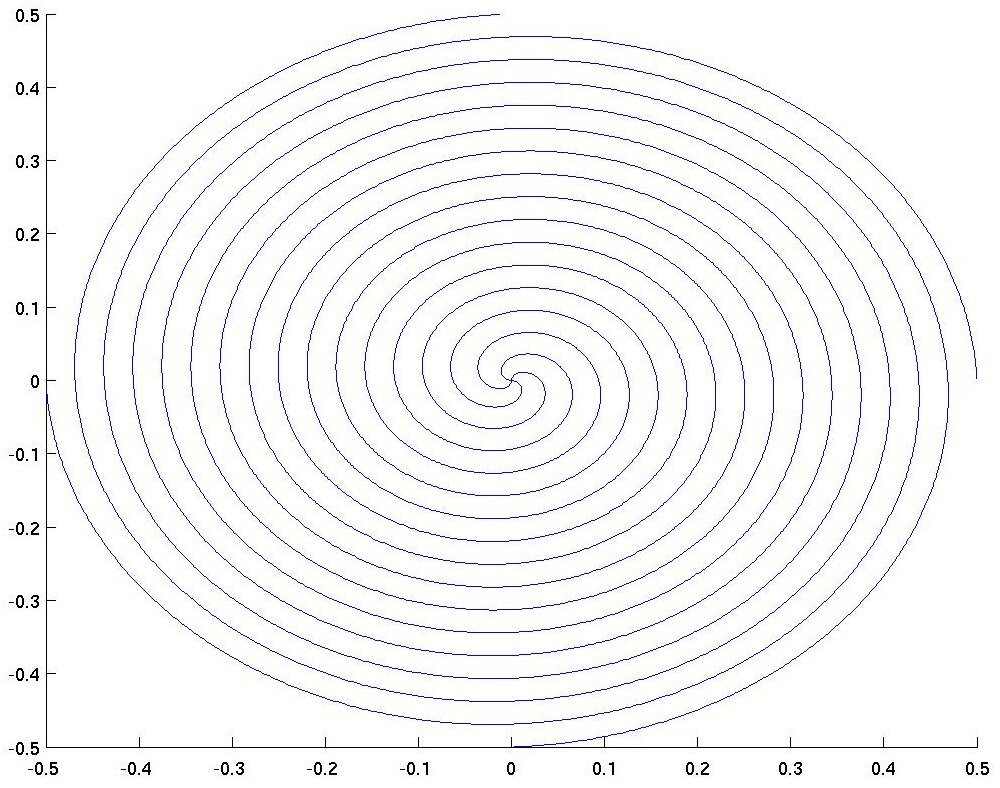
\includegraphics[width=5.5cm]{pics/spiral.jpg} &
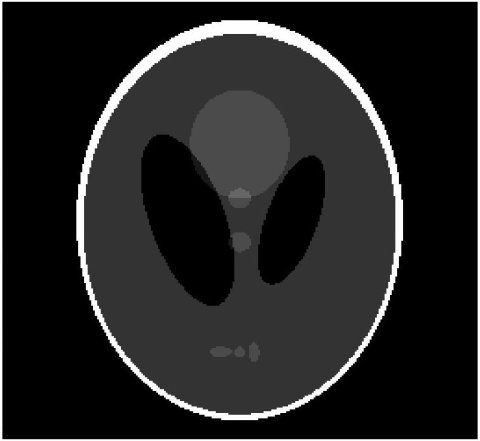
\includegraphics[width=5.5cm]{pics/phantom_original.jpg} &
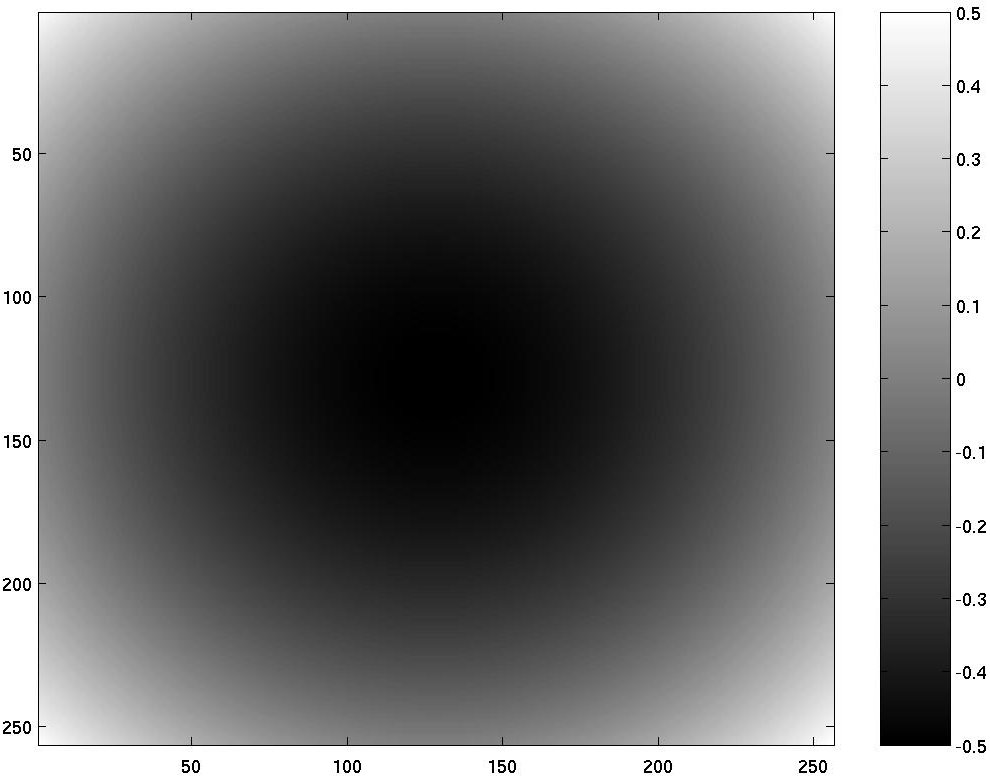
\includegraphics[width=5.5cm]{pics/fieldmap_simulated.jpg}
\end{tabular}
\caption{A subset of the k-Space trajectory, here with only 4 interleaved spiral arms (left), the used phantom (middle) and the simulated field map (right)}
\label{Fig:Phantom}
\end{figure*}

\begin{table}[ht]
\begin{center}
\begin{tabular}{|l||c|c|c|c|c|} \hline
 \rule{0mm}{4mm} method $\backslash$ iter. & $1$ & $2$  & $5$  & $10$ &  \\[1ex] \hline\hline
 \multicolumn{5}{|c|}{\rule{0mm}{4mm} SNR}& \\[1ex] \hline\hline
 \rule{0mm}{4mm} Gridding &  &  &  &  & \\[1ex] \hline
 \rule{0mm}{4mm} 3d NNFFT &  &  &  & &  \\[1ex] \hline
 \rule{0mm}{4mm} 3d NFFT &  &  &  &  & \\[1ex] \hline
 \rule{0mm}{4mm} 2d$\otimes$1d NFFT &  & &  & &  \\[1ex] \hline \hline
 \multicolumn{5}{|c|}{\rule{0mm}{4mm} CPU-Time} &Memory in MB \\[1ex] \hline\hline
 \rule{0mm}{4mm} Gridding &  &  &  & &  \\[1ex] \hline
 \rule{0mm}{4mm} 3d NNFFT &  &  &  &  & \\[1ex] \hline
 \rule{0mm}{4mm} 3d NFFT &  &  &  &  & \\[1ex] \hline
 \rule{0mm}{4mm} 2d$\otimes$1d NFFT &  & &  & &  \\[1ex] \hline \hline

\end{tabular}
\end{center}
\caption{SNR and CPU-time for different reconstruction methods after $1$, $2$, $5$, and $10$ iterations.} \label{Tab:1}
\end{table}

\textbf{Numerical Experiment 1:}


fieldmap

Wie wurde die fieldmap berechnet? siehe Fessler?

\begin{figure*} 
\centering
\begin{tabular}{c}
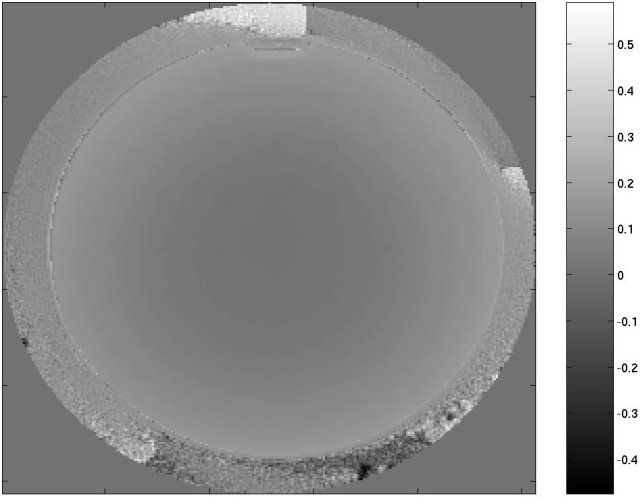
\includegraphics[width=7cm,height=6cm]{pics/fieldmap.jpg} 
\end{tabular}
\caption{The measured field map (left) in kHz.}
\label{Fig:Philips}
\end{figure*}


\begin{figure*}[ht] 
\centering
\begin{tabular}{cc}
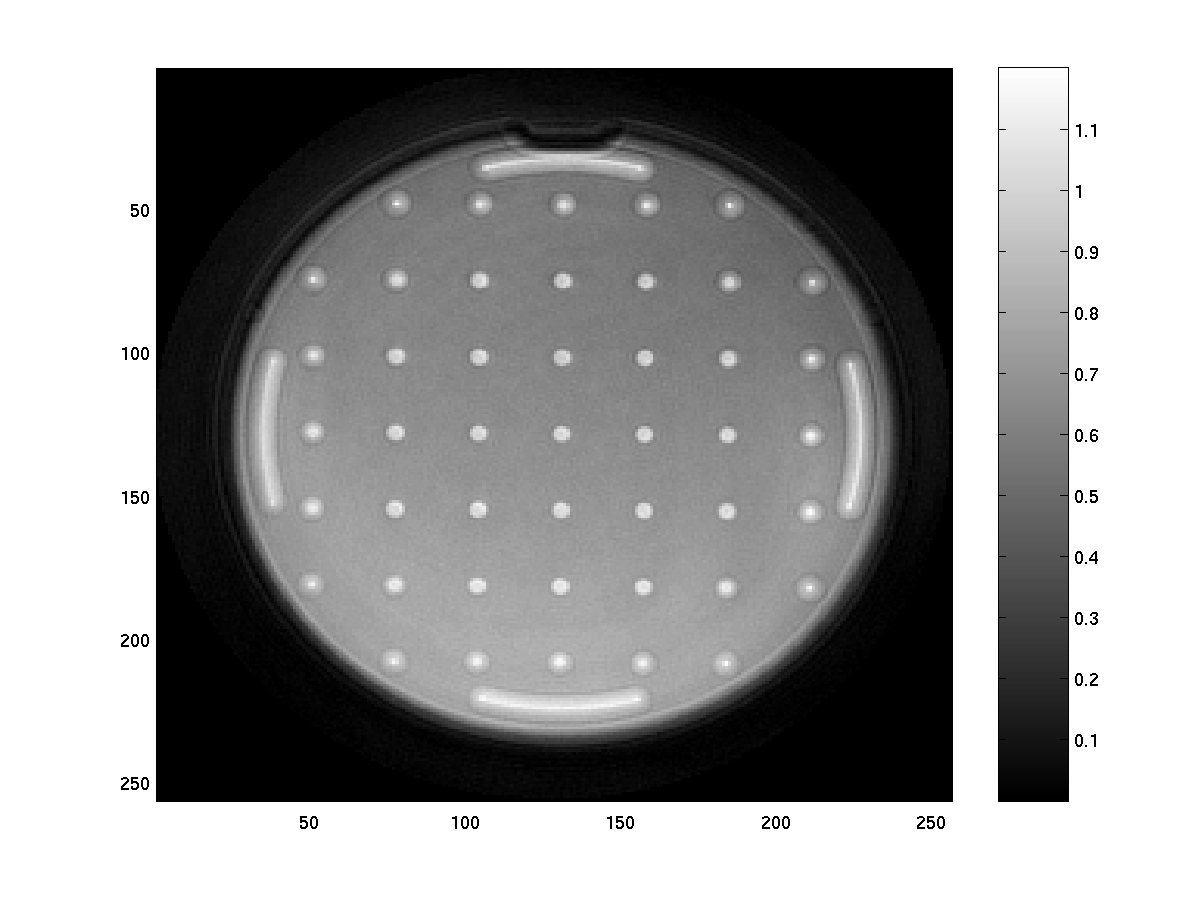
\includegraphics[width=7cm]{pics/reallife_400_gridding_iter=1.png} &
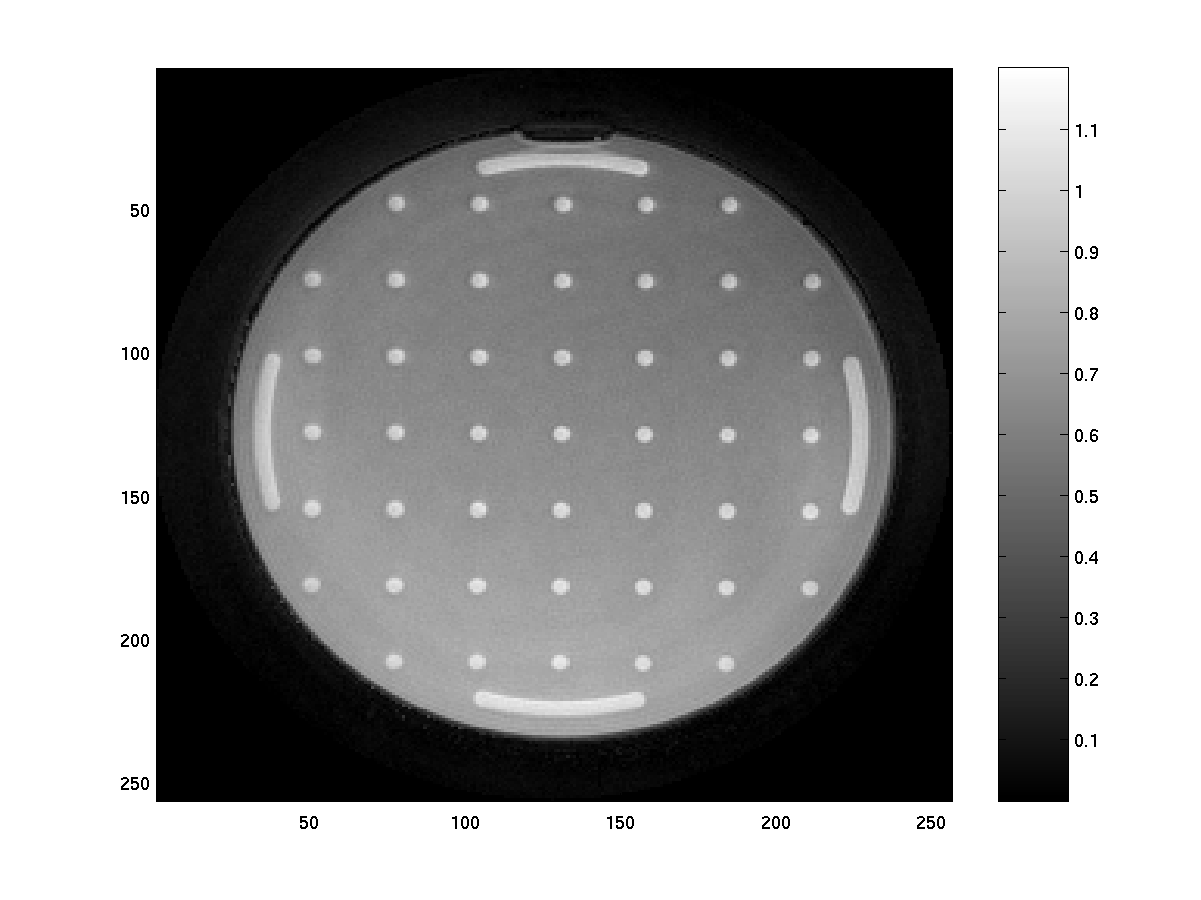
\includegraphics[width=7cm]{pics/reallife_400_iter=1.png}\\
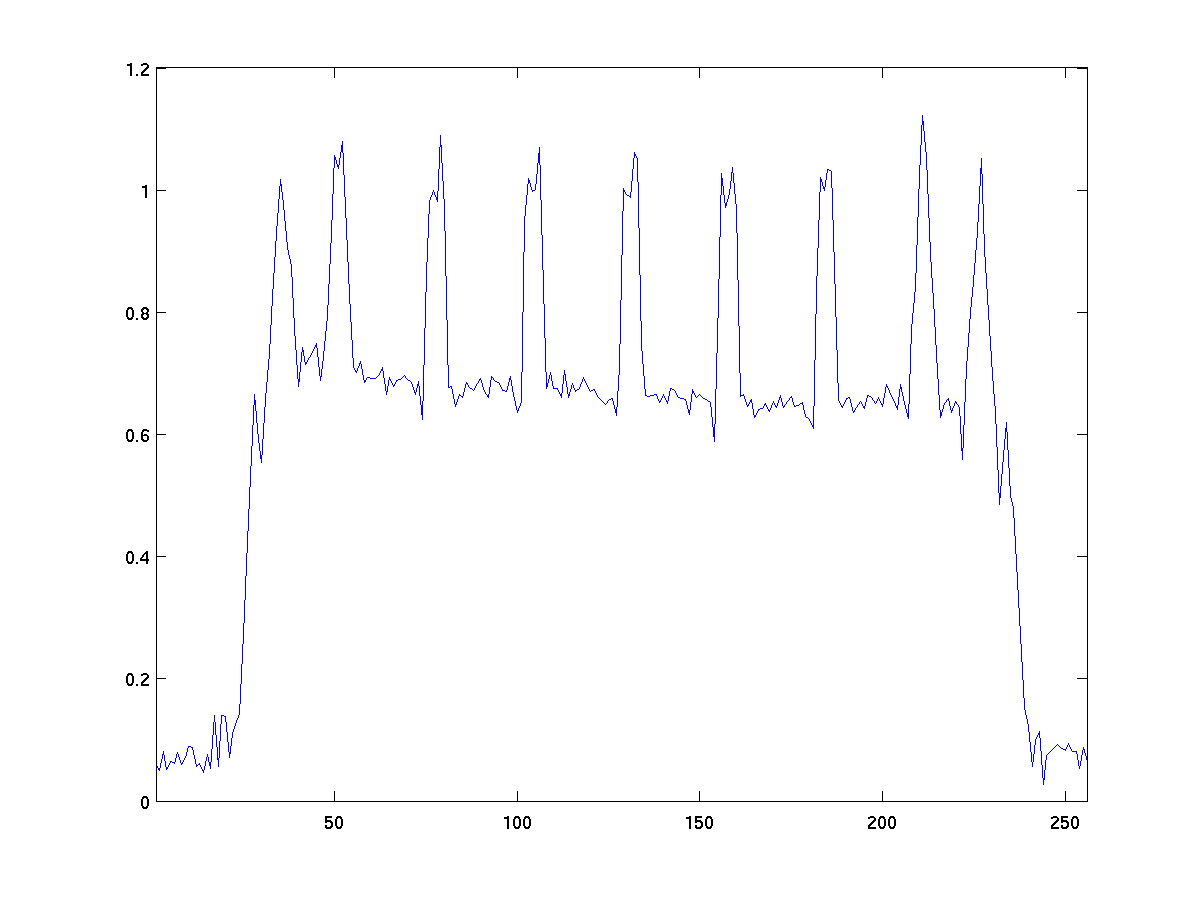
\includegraphics[width=7cm]{pics/reallife_400_gridding_iter=1row.png} &
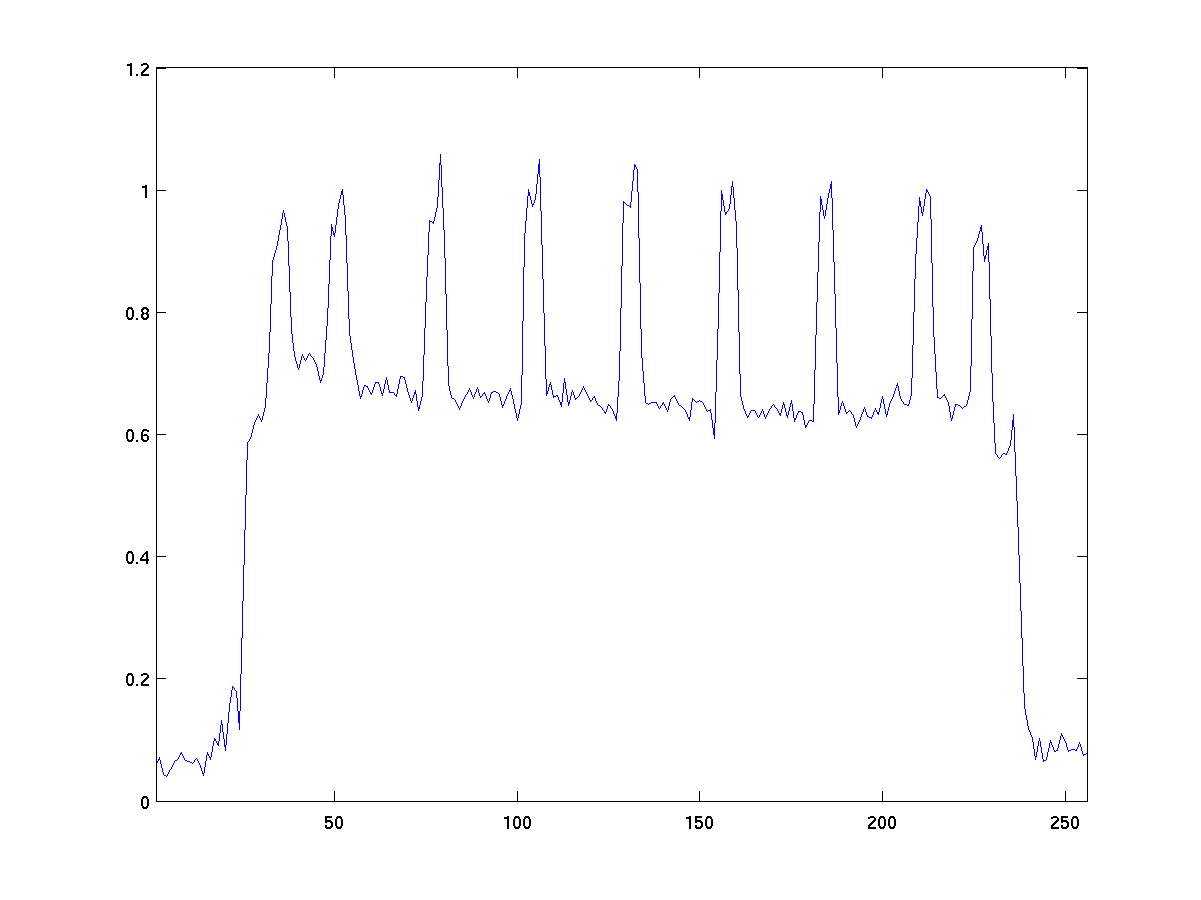
\includegraphics[width=7cm]{pics/reallife_400_iter=1row.png}
\end{tabular}
\caption{Physical phantom from a MR scan by the Philips Achieva 1.5T device, reconstructed
with gridding (left) and 2d$\otimes$1d NFFT (right) after one iteration}
\label{Fig:Philips}
\end{figure*}

\begin{figure*}[ht] 
\centering
\begin{tabular}{cc}
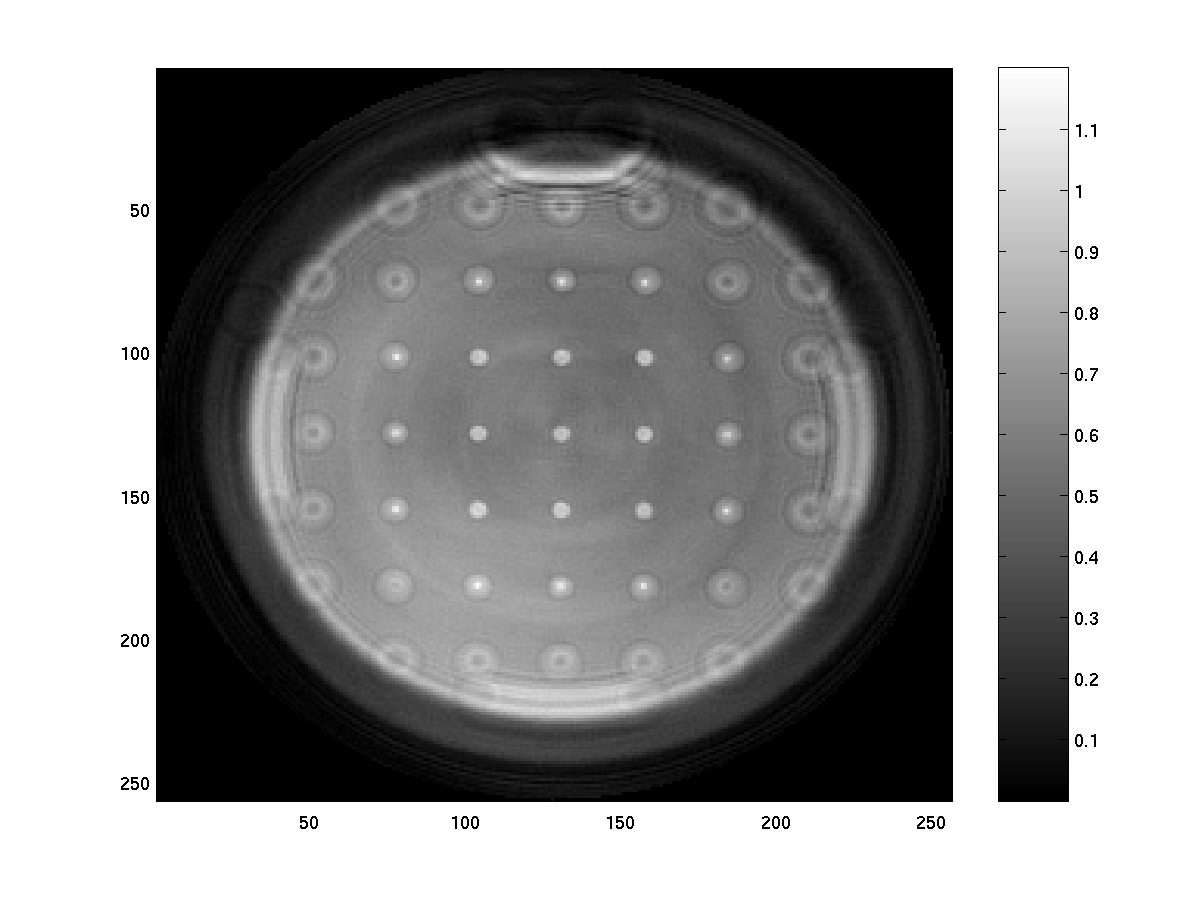
\includegraphics[width=7cm]{pics/reallife_900_gridding_iter=1.png} &
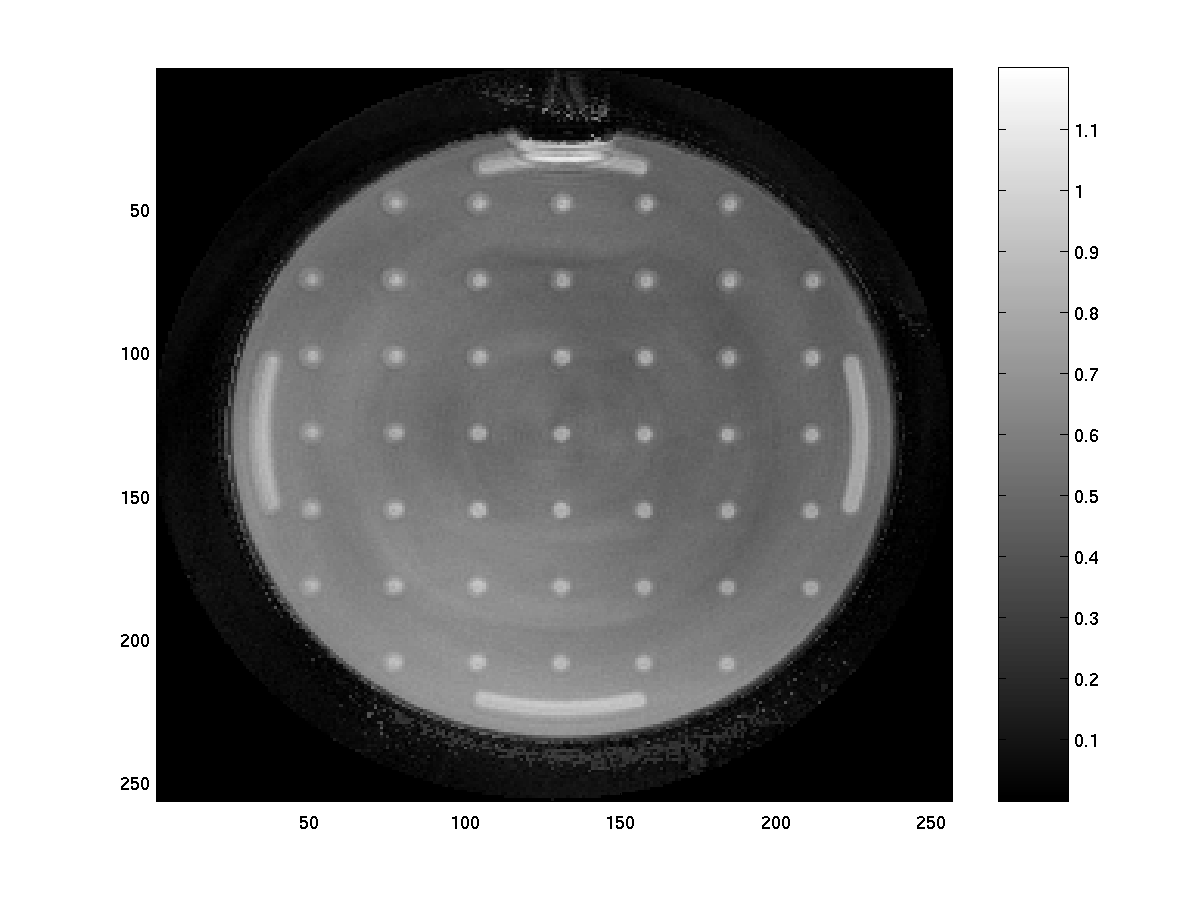
\includegraphics[width=7cm]{pics/reallife_900_iter=1.png}\\
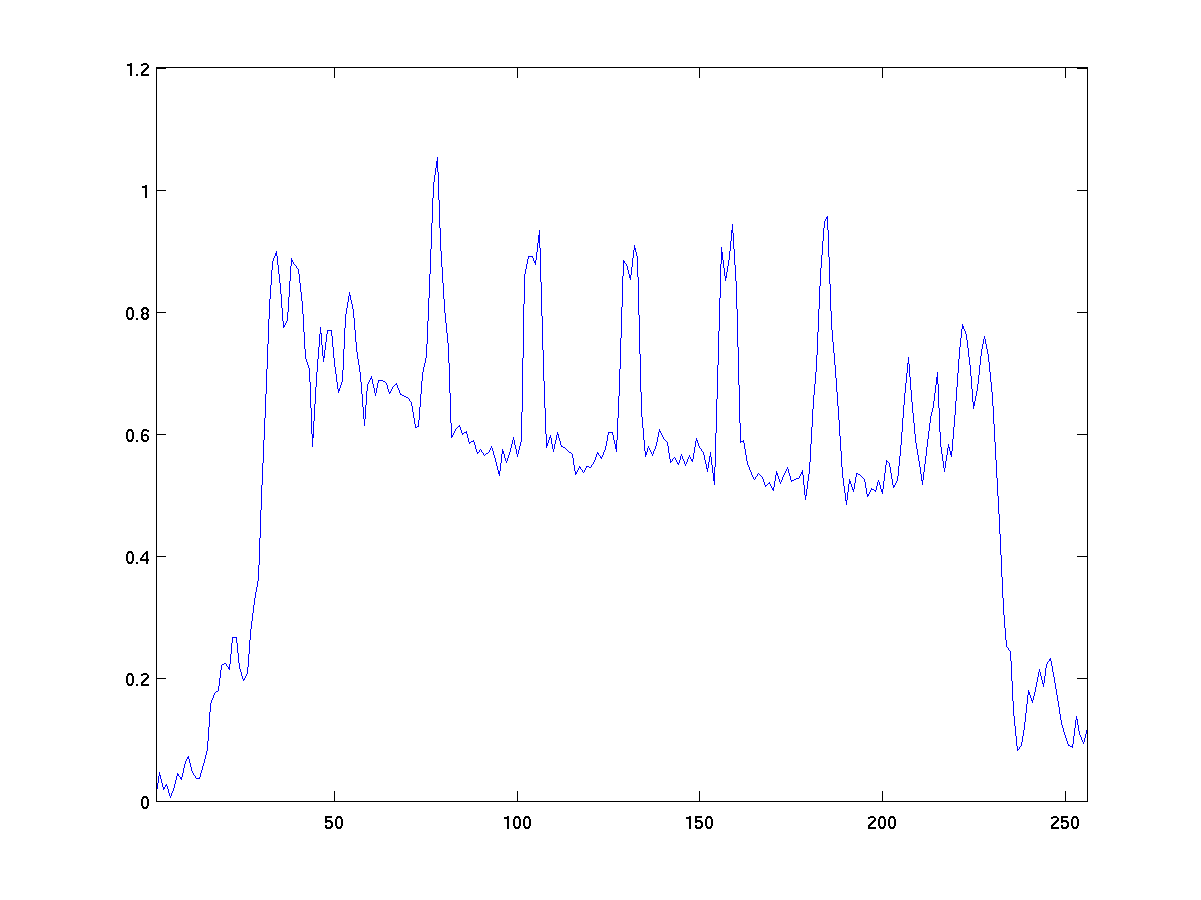
\includegraphics[width=7cm]{pics/reallife_900_gridding_iter=1row.png} &
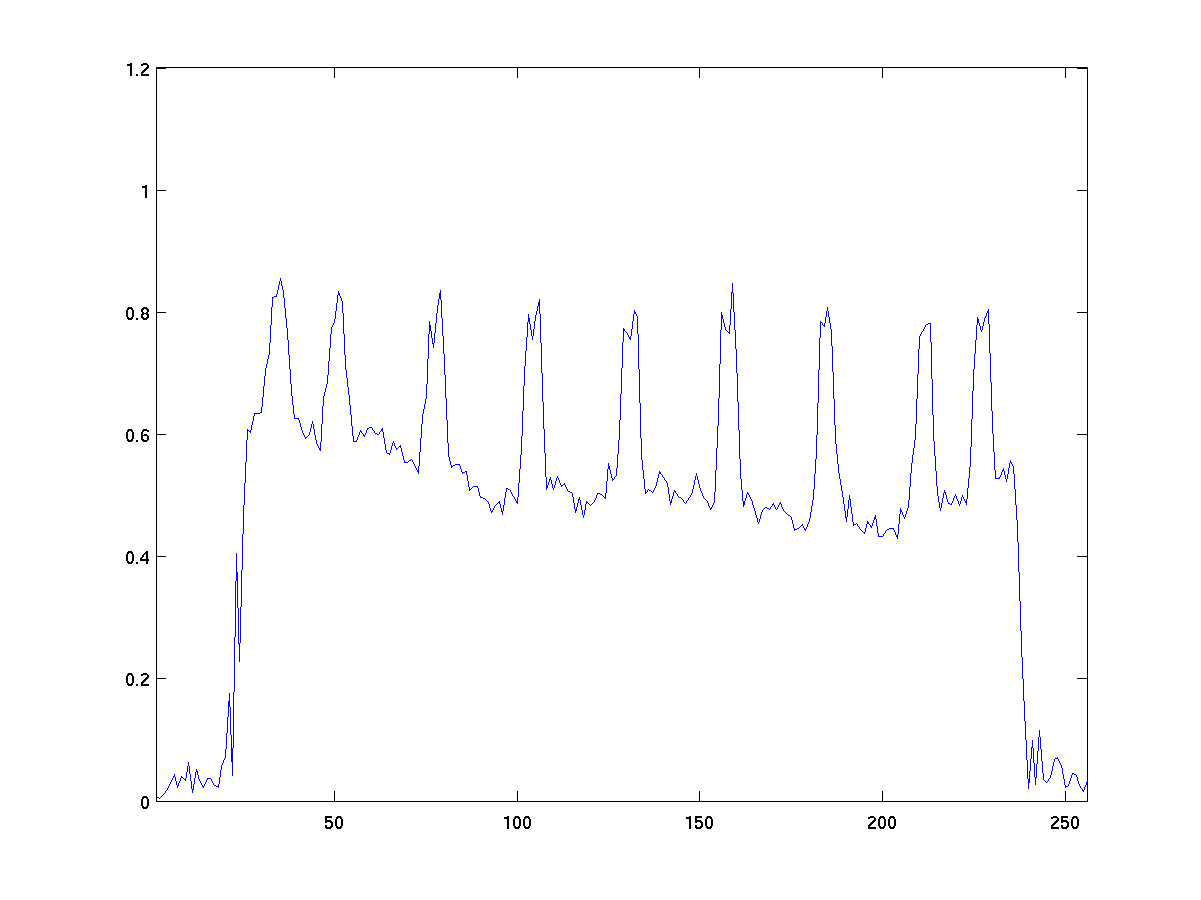
\includegraphics[width=7cm]{pics/reallife_900_iter=1row.png}
\end{tabular}
\caption{Two slices of the reconstruction with Voronoi weights after one iteration from a MR scan by the Philips Achieva 1.5T device.}
\label{Fig:Philips}
\end{figure*}



% \begin{figure*}[ht] 
% \centering
% \begin{tabular}{cc}
% \includegraphics[width=7cm,height=6cm]{/home/ana/knopp/nfft_programs/philipsdaten_inhomo/pics_png/phantom_inh.jpg} &
% \includegraphics[width=7cm,height=6cm]{/home/ana/knopp/nfft_programs/philipsdaten_inhomo/pics_png/phantom_gridding.jpg} 
% \end{tabular}
% \caption{phantom-inh.jpg (links), phantom-gridding.jpg (rechts)}
% \label{Fig:Philips}
% \end{figure*}
% 
% \begin{figure*}[ht] 
% \centering
% \begin{tabular}{cc}
% \includegraphics[width=7cm,height=6cm]{/home/ana/knopp/nfft_programs/philipsdaten_inhomo/pics_png/bild_gridding.png} &
% \includegraphics[width=7cm,height=6cm]{/home/ana/knopp/nfft_programs/philipsdaten_inhomo/pics_png/bild_inhomog.png} 
% \end{tabular}
% \caption{bild-gridding.png (links), bild-inhomog.png (rechts)}
% \label{Fig:Philips}
% \end{figure*}
% 
% \begin{figure*}[ht] 
% \centering
% \begin{tabular}{cc}
% \includegraphics[width=7cm,height=6cm]{/home/ana/knopp/nfft_programs/philipsdaten_inhomo/pics_png/bild_gridding_philips.png} &
% \includegraphics[width=7cm,height=6cm]{/home/ana/knopp/nfft_programs/philipsdaten_inhomo/pics_png/bild_iter=5_philips.png} 
% \end{tabular}
% \caption{bild-gridding-philips.png (links), bild-iter=5-philips (rechts)}
% \label{Fig:Philips}
% \end{figure*}

{\bf Acknowledgement.}

%\bibliographystyle{IEEEabbrv}
%\bibliographystyle{IEEEtran}
%\bibliography{/home/knopp/Uni/Studienarbeit/ref}
\end{document}
